\UseRawInputEncoding
\documentclass[12pt]{article}
\title{ECE 141 Homework 4}
\usepackage{subcaption}
\author{Lawrence Liu}
\usepackage{graphicx}
\usepackage{amsmath}
\usepackage{placeins}
\newcommand{\Laplace}{\mathscr{L}}
\setlength{\parskip}{\baselineskip}%
\setlength{\parindent}{0pt}%
\usepackage{xcolor}
\usepackage{listings}
\definecolor{backcolour}{rgb}{0.95,0.95,0.92}
\usepackage{amssymb}
\lstdefinestyle{mystyle}{
    backgroundcolor=\color{backcolour}}
\lstset{style=mystyle}

\begin{document}
\maketitle
\subsection*{Problem 5.5}
\subsection*{(c)}
$L(s)$ has zeros at $\frac{-2\pm j2\sqrt{7}}{2}$, and poles at $0$ and $\frac{-2\pm j6}{2}$, therefore we have $\alpha=0$
$\phi_{1}=180^{\circ}$, 
And the departure angle for poles $-1\pm3j$ is $\pm161.565^{\circ}$, And the arival angle for the zeros $-1\pm\sqrt{7}j$ is $\pm200^{\circ}$\\\\
Therefore the sketch fo the root locus looks like the following
\\
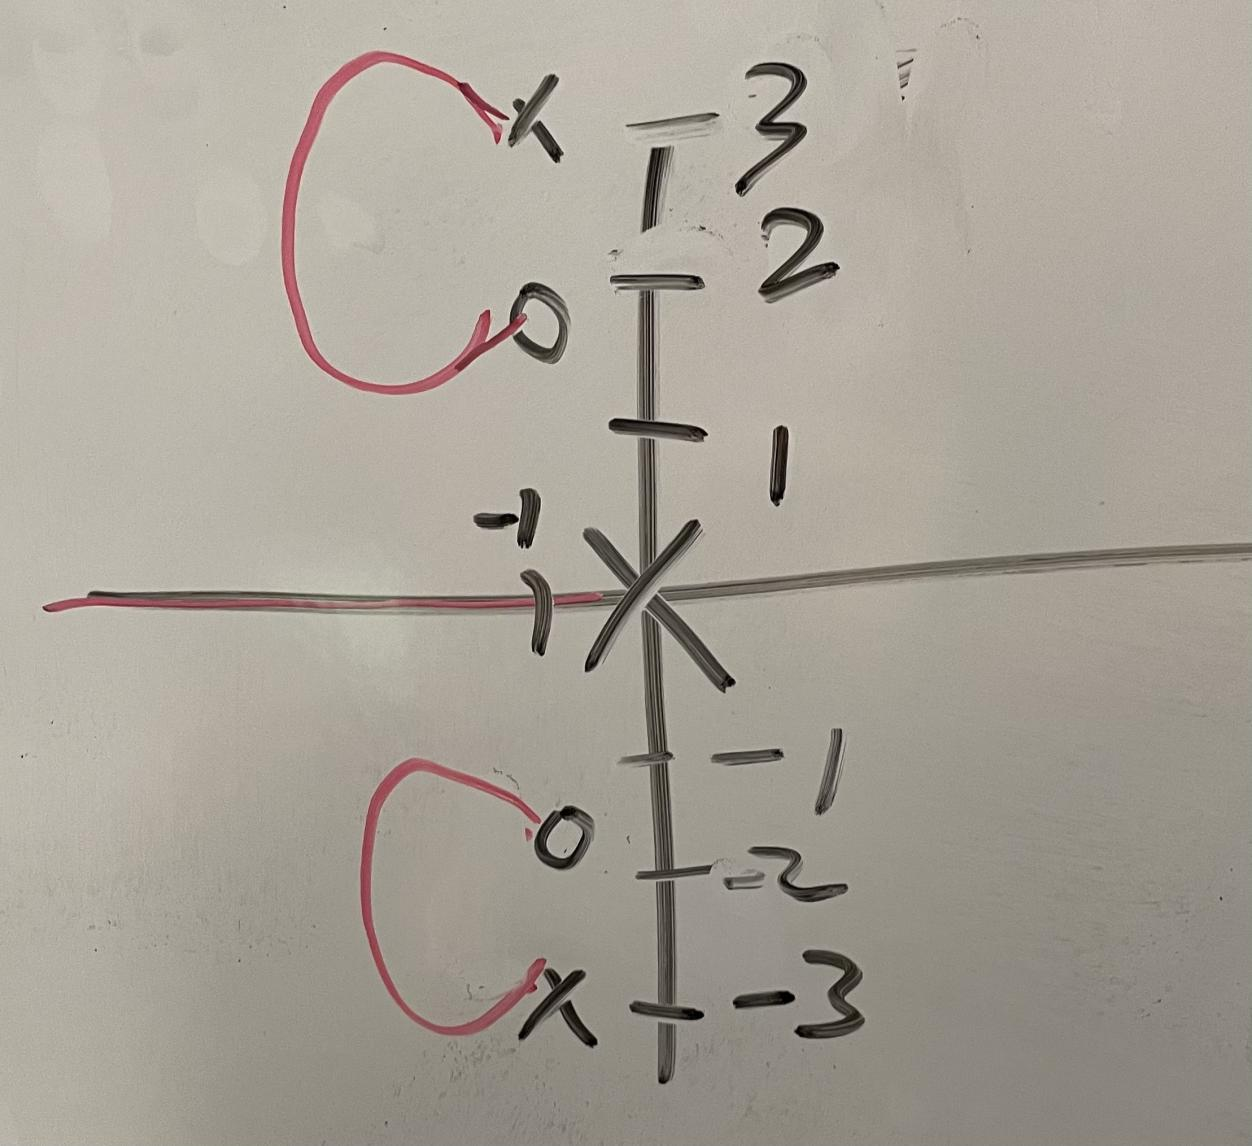
\includegraphics[scale=.15]{Problem1Sketch1.jpg}
\\Matlab code to do as well

\subsection*{(e)}
$L(s)$ has zeros at $\pm j$, and poles at $0$ and $\pm4j$, therefore we have $\alpha=0$
$\phi_{1}=180^{\circ}$, 
And the departure angle for poles $\pm2j$ is $180^{\circ}$, And the arival angle for the zeros $\pm1j$ is $180^{\circ}$\\\\
Therefore the sketch fo the root locus looks like the following
\\
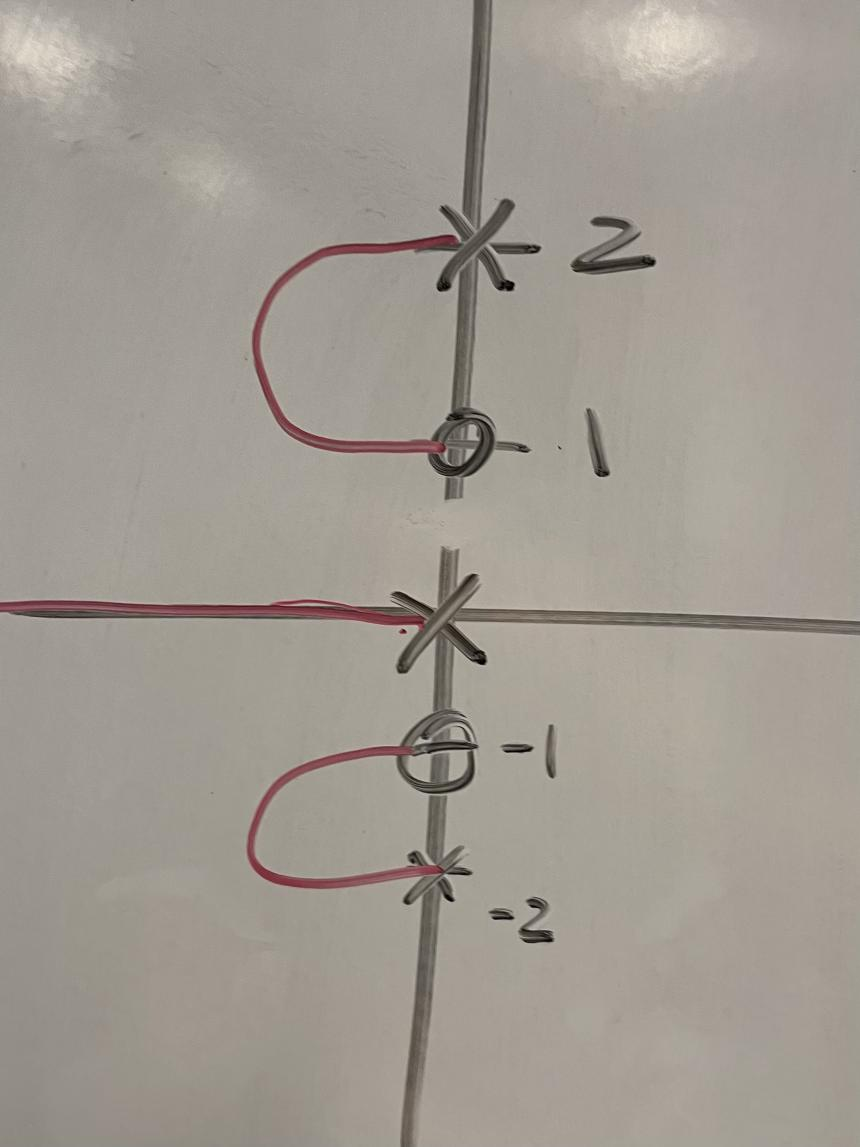
\includegraphics[scale=.15]{Problem1Sketch2.jpg}
\\
Matlab code to do as well
\section*{Problem 5.7}
\subsection*{(c)}
This functions has 2 zeros at $-3$ and 5 poles: 2 at $0$, 1 at $-10$, and 2 at $-3\pm\frac{5j}{2}$
Therefore $\alpha=-3.333$ and 
\end{document}